\documentclass[conference]{IEEEtran}
\IEEEoverridecommandlockouts
% The preceding line is only needed to identify funding in the first footnote. If that is unneeded, please comment it out.
\usepackage{amsmath,amssymb,amsfonts}
\usepackage{algorithmic}
\usepackage{graphicx}
\usepackage{textcomp}
\usepackage{xcolor}
\usepackage[backend=biber,style=ieee,autocite=inline]{biblatex}
\bibliography{ref.bib}
\DefineBibliographyStrings{english}{%
  bibliography = {References},}
\def\BibTeX{{\rm B\kern-.05em{\sc i\kern-.025em b}\kern-.08em
    T\kern-.1667em\lower.7ex\hbox{E}\kern-.125emX}}
\begin{document}

\title{Applications of NLP in detecting transitional words in text\\
}

\author{\IEEEauthorblockN{Ilya Nokhrin}
\IEEEauthorblockA{\textit{dept. name of organization (of Aff.)} \\
\textit{name of organization (of Aff.)}\\
City, Country \\
email address or ORCID}
\and
\IEEEauthorblockN{Moofiy Imam}
\IEEEauthorblockA{\textit{dept. name of organization (of Aff.)} \\
\textit{name of organization (of Aff.)}\\
City, Country \\
email address or ORCID}
}

\maketitle

\begin{abstract}
Many ongoing projects require to process raw text in various ways. Traditionally, manual processing and text mining were the primary methods used for this purpose. However, the advancement of neural networks in recent times has introduced NLP as an alternative and effective approach for tackling such tasks. We confirmed this by studying current scientific works, as numerous existing studies have demonstrated successful implementations of NLP to address their specific requirements.

After we have proven that NLP is successfully applicable to natural language processing tasks, we have devised our own solution to address a previously unexplored issue: the detection of transition words in a given text using NLP application build on Python with spaCy library. Model has proven to successfully perform that task, with all of the metrics exceeding 80\%, though future improvement is also discussed. We also explore some of the possible applications of the model, including analysis of academic writing for educational purposes.
\end{abstract}

\begin{IEEEkeywords}
AI, machine learning, natural language processing, NLP, spaCy, extractive analysis, semi-structured data
\end{IEEEkeywords}

\section{Introduction}

In the present day, accessibility and power of artificial intelligence grow with every day. AI is applied in a variety of fields. If, for instance, we consider software engineering, AI tools can be used at almost every step of the process: requirement elicitation \cite{intro-1}, development \cite{intro-2}, testing \cite{intro-3} and customer service \cite{intro-4}. 

Of these applications, ones that stand out are these which require to process text - and not the uniform type of text like code in a particular programming language or sanitized data set, but natural language, such as elicited requirements, text-based feedback or text from a scientific paper. 

For these cases, a technology known as natural language processing (NLP) is often used \cite{intro-5}. NLP is a subfield of AI that focuses on enabling machines to understand, interpret, and generate human language. Its main application is analyzing and processing natural language data to extract certain information - for instance, patterns or tokens (i.e. locations, names or numbers). 

In the following chapters, we will discuss existing applications of NLP in language processing and provide a solution to one particular issue - detecting transitional words in a given scientific text. 

\section{Literature review}

\subsection{NLP applications in software engineering}

When it comes to software engineering, NLP is mostly applied to documentation, requirements and feedback, as these are the artifacts that are usually represented in the form of a natural text.

Di Sorbo, Visaggio, Di Penta, Canfora and Panichella \cite{lr-1} identified that processing unstructured artifacts is useful for development of suggester systems (which, in turn, help in several different ways, such as extracting action points from user feedback and generating documentation). However, such processing requires a manually-specified ruleset. To mitigate this, researchers used NLP and created a system that can produce rules automatically, with more than a third of rules generated by their system being relevant for a specified task.

Al Omran and Treude \cite{lr-2} discuss application of NLP to software documentation in multiple forms (such as StackOverflow data and GitHub ReadMe files) and conclude that this application of NLP can lead to a discovery of useful and actionable information, but requires justification (as certain actions could be performed more efficiently by approaches such as text mining) as well as informed choice (and, potentially, further customization) of an NLP library.

Ferrari and Esuli \cite{lr-3} discuss how the ambiguity during the requirement elicitation process can negatively affect later stages of development and propose an NLP-based solution to this problem. A model was created for each area of stakeholders' expertise and later used to automatically detect and score ambiguity of terms with varying meanings in different areas. This approach was found to be applicable to most of the scenarios in which it was tested.

Joshi and Deshpande \cite{lr-4} proposed that current tools for automatic generation of UML diagrams from natural language requirements are inefficient and developed an NLP-based tool called RAUE that implements natural language processing for extracting data for UML diagram generation. This tool was able to successfully detect all types of relations between entities with an accuracy of about 85\% (based on precision and recall metrics).

\subsection{NLP applications in text analysis}

When it comes to text analysis, NLP is used in two major ways: either for sentiment analysis (mostly as one step in the process - i.e. tokenization) or for extractive analysis.

\subsubsection{Sentiment analysis}
Sentiment analysis is mostly concerned with what is the general meaning of a particular text. These approaches try to abstract from the text in general towards the intent of the author. In these cases, NLP is mostly used as a tokenizer or in other data cleanup approaches.

Rameshbhai and Paulose \cite{lr-5} discuss one such application of NLP - newspaper headlines opinion mining. In this paper, NLP is used for tokenization of data to later on be processed manually and later produce a model using SVM.

Hasan, Maliha and Arifuzzaman \cite{lr-6} also use NLP in sentiment analysis. Here, NLP is used to clean data as well as to detect and remove stop-words. After sanitizing data in this way, other techniques, such as Bag of Words (BoW) and Term Frequency-Inverse Document Frequency (TF-IDF) are used for the sentiment analysis itself.

\subsubsection{Extractive analysis}
Extractive analysis is, as name would suggest, largely focused on extracting data from provided text and compiling it in a certain way. Here, applications of NLP are of much greater variety, as a lot of data can be extracted from text using NLP (part-of-speech data, lemmas, tokens, etc.).

Hendrycks, Burns, Chen and Ball \cite{lr-7} concluded that there are a lack of domain-specific datasets, and created Contract Understanding Atticus Dataset (CUAD) - a dataset of other 13000 manually written annotations, which is created with the purpose of highlighting important parts of legal contracts for a human to review. In addition to its main purpose, CUAD is usable as a benchmark for domain-specific NLP models.

Carchiolo, Longheu, Reitano and Zagarella \cite{lr-8} applied NLP to process scanned medical prescriptions. Their implementation does so by extracting embedded terms and then comparing them against patient and doctor personal data, symptoms, diagnosis and proposed treatment. Resulting system was able to automatically classify 95\% of prescriptions as either grantable or not.

Sarica, Song, Low and Luo \cite{lr-9} proposed an approach to improve grant search. They use NLP to train a model, which is later used to rank keywords in the patent information. This way, the system can provide a list of a potentially relevant terms to include in the future searches, which allows users to greatly improve their searching progress. Moreover, this system also provides groups of keywords that are relevant to the topic only in combination with each other, but not by themselves.

Lastly, Kauchak, Leroy, Pei and Colina \cite{lr-10} discuss a topic that is the closest in scope to that of this paper: predicting transitional words between pairs of sentences. They considered two questions for a given pair of sentences: whether a transition should be used at all and, if it is, which one would fit the context the most. Work was performed for English and Spanish languages, and average accuracy of transitional word choice were 78\% and 84\%, respectively.

\subsection{Takeaways}

Based on the existing work research, following conclusions can be drawn:
\begin{enumerate}
    \item NLP has been used in a variety of text-analysis scenarios to a relatively high success
    \item NLP shows best results when applied to problems which require detection of words relevant to a specific topic or category
    \item While relatively accurate, NLP-based solutions have accuracy that is in the range of 75-85\%, becoming lower in the particularly niche cases. That means, that in simpler projects other approaches might be preferable for greater accuracy, but NLP offers one of the greatest flexibility when it comes to data.
\end{enumerate}

This work is also relevant, because while each of the points stated below has been addressed at least once, there are no research which covers all of them at once:

\begin{enumerate}
    \item Using NLP for extractive analysis
    \item Applying extractive analysis to research papers
    \item Detecting a particular non-standard (not covered by pre-trained models) token (transitional word, in this case)
\end{enumerate}

\section{Implementation}
To train the model, following steps had to be taken:
\begin{itemize}
    \item Decide on the implementation: which libraries have to be used, which models are we planning to use and produce as the result of this project.
    \item Process transition words data. In this step, we take initial transitions set in a CSV format, process and clean it, and then handle complex transition cases (i.e. transitions consisting on multiple words)
    \item Generate training data based on sanitized sample text and processed transition words. In this step, we update existing spaCy model with new entities - transitions extracted in the previous step, and use this model to process sanitized data and produce training data (so-called gold standard)
    \item Train the model using generated training data. In this step, we train the model using spaCy’s training module and the gold standard produced in the previous step. After this step, our result model is ready to be used
    \item Run the model. In this step, we process data previously unused in the training process to test our model
    \item Assess produced results and relevant metrics. In this step, we compare produced result to the gold standard and use the result to generate confusion matrix, as well as model metrics (accuracy, precision, recall and F1)
\end{itemize}

\subsection{General project information}
In the implementation of the project, following libraries were utilized:
\begin{itemize}
    \item spaCy is the NLP library of choice for this project. It is used for the majority of the steps listed above. It was chosen over NLTK due to several advantages:
    \begin{itemize}
        \item SpaCy has faster text processing speed compared to NLTK
        \item NLTK is string based, as opposed to object-based. Processing tokens as objects simplifies the training process and visualization (as all of the data relevant to the token is stored in a simple to access way)
    \end{itemize}
    \item displacy is the module of spacy that is used to output formatted data. It is mostly used for visualization
    \item random is a standard python library. It is used to shuffle training data during the process of model training
    \item json library is used to save and load intermediary data
\end{itemize}

During the course of the project two NLP models are used:
\begin{itemize}
    \item en\_core\_web\_md is the default medium-size english model provided with spaCy. A medium size model is used to strike a balance between speed of use and robustness
    \item transition\_ner is the intermediary model based on the default spaCy model with added entities for labels
    \item transitions\_ner\_model is the model trained during the course of the project
\end{itemize}

\subsection{Process transition words data}
The first step was to process transition words provided to use later on. Originally words were provided in the csv (comma-separated values) format:

\begin{figure}[htbp]
\begin{center}
    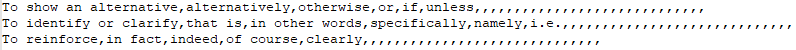
\includegraphics[width=0.45\textwidth,height=\textheight,keepaspectratio]{images/csv.png}
\end{center}
\caption{Raw data in CSV format}
\label{fig_csv}
\end{figure}

To process this file, several steps were taken, which could be roughly separated into 3 blocks:

\begin{itemize}
    \item Reading and cleaning file
    \item Processing elements with word variations
    \item Processing elements with word omissions
\end{itemize}

Implementations of listed steps are shown in the image above. 

\begin{figure}[htbp]
\begin{center}
    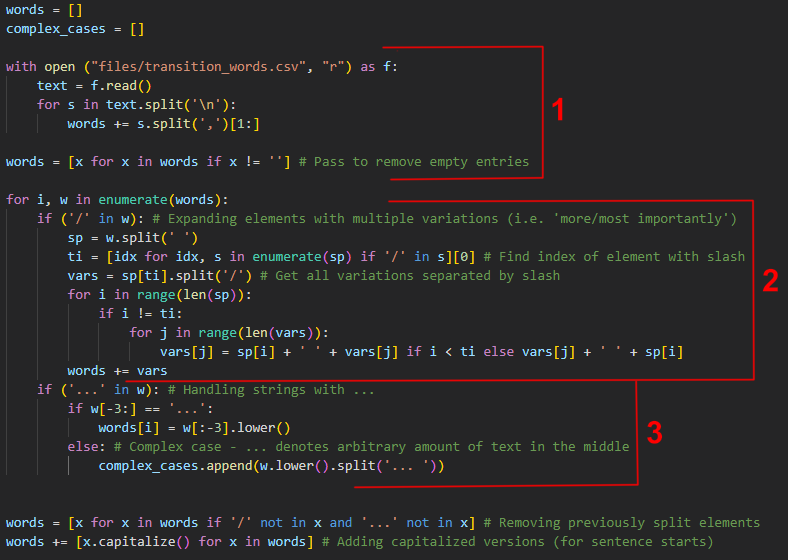
\includegraphics[width=0.45\textwidth,height=\textheight,keepaspectratio]{images/listing1.png}
\end{center}
\caption{Code for processing data}
\label{fig_listing1}
\end{figure}

In the first block, we open the file, read the data from it, and then split values on line feeds (\\n) and commas. When we split the file based on commas, empty values are generated (as seen on screenshot of initial data, there are multiple trailing commas, which contain empty values after the split), so we remove those in the last step. We also remove the first entry in each row, as it contains the name of the transition word category, and is not used.

By the end of the first block, certain values are already processed and ready to be used. Those are single word (i.e. similarly, equally) or multiple word (i.e. as a consequence) values In the second block, we process one of the more complex cases - values with multiple word variations (i.e. more/most importantly). To do that, we first find the index of an element with multiple variations (via it containing a slash character). After that, we split this element to obtain all of the word variations. As a final step, we go through the original value, substitute the element containing multiple variations with a particular variation and add it to the result array. This is performed for each of the variations.

In the next block another complex case is processed - elements with omitted words (i.e. It is clear that...). There are two possible cases of such elements: they either contain “...” at the end of the sentence (in which case it is simply trimmed from the element) or they contain “...” in the middle of the sentence (in that case, an array of two elements - part before and part after the dots, - is added to the complex\_cases array. It’s not currently used, but might be implemented in the future).

After these blocks, two more operations are performed on the array: all of the previously processed complex cases are removed and capitalized versions of every entry is added (to detect entries at the start of the sentence)

\subsection{Generating training data}
In the next step, we use prepared transition words to update existing spaCy model with new entities and use this model to process sanitized data, producing training data used in the next steps as a result

Code for this step can also be separated into 3 blocks:

\begin{itemize}
    \item Update existing model with new entities
    \item Load the text
    \item Process loaded text using the updated model
\end{itemize}

\begin{figure}[htbp]
\begin{center}
    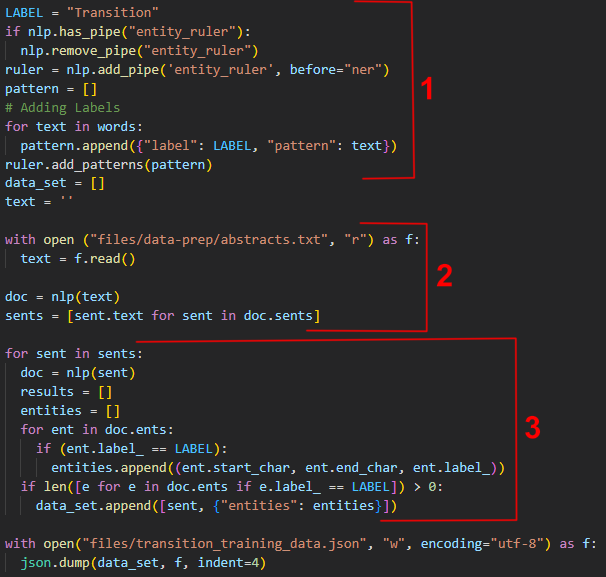
\includegraphics[width=0.45\textwidth,height=\textheight,keepaspectratio]{images/listing2.png}
\end{center}
\caption{Code for generating training data}
\label{fig_listing2}
\end{figure}

In the first block, we specify the name of a new label. Then we remove and re-add the necessary processing step (called “pipe” in spacy) to ensure that it is present, but not duplicated in the pipeline. After that we add all of our transition words in a special format used by spaCy (a Python dictionary with keys for label - category of added word, and pattern - specific word or regular expression to match).

In the second block, we load the text and split it into sentences using spaCy

In the third step, we process each sentence by finding all of the entities contained in it (both entities from the default model and our transition entities). We then record start position, end position and label of each of the transitions (this is the format of the annotation used in the data set later on). Then we append a list consisting of the sentence and dictionary containing annotations for all of the transition entities found in this sentence (if none were found, the sentence is omitted)

Finally, we export the resulting data in the JSON format to be used later

\subsection{Training the model}
In this step, all of the data is prepared and the model is ready to be trained. This step consists of 2 blocks of code:

\begin{itemize}
    \item Create and prepare empty model
    \item Train the model
\end{itemize}

\begin{figure}[htbp]
\begin{center}
    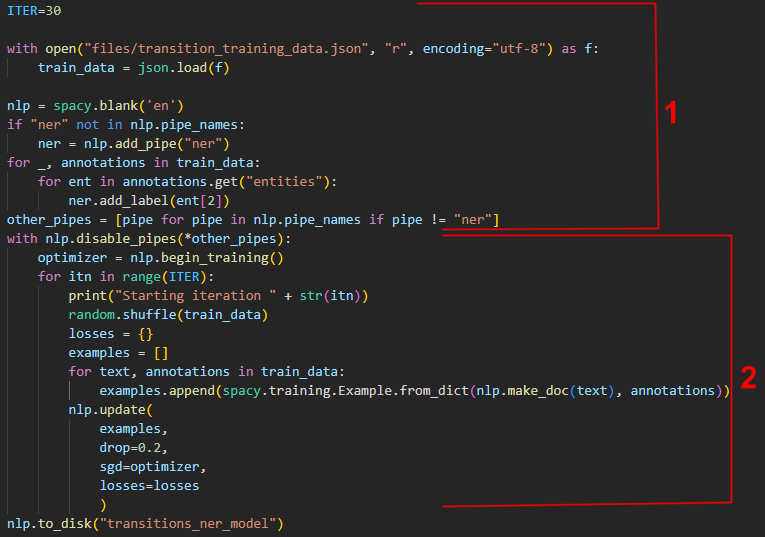
\includegraphics[width=0.45\textwidth,height=\textheight,keepaspectratio]{images/listing3.png}
\end{center}
\caption{Code for model training}
\label{fig_listing3}
\end{figure}

In the first block we load our previously prepared training data. After that, we create a new empty model. The only pipe used in it is ner (named entity recognition). We add labels to be recognised (in this particular case it’s only the “Transition” label, but this code can accommodate additional labels if needed).

At the start of the second block, we disable all of the other pipes except for “ner”, and then start the training process. The training process basically consists of using the model to process a sentence in the text form and then compare it to the gold standard annotations. Then, based on the examples produced that way (using spaCy’s training.Example.from\_dict method), the model is updated and one training iteration is finished. In total, this training session took 30 iterations.

After the model is trained, it is saved to the disk. From this moment, it can be imported and used just as default spaCy models

\subsection{Running the model}
By this point, we can run the model on a text that was not used in the previous training (and thus, completely unknown by the model) and successfully detect transition words in the sentences. Example of processed data (formatted using displacy library) is shown below. Each of the highlight words was classified as a transition by our newly trained model.

\begin{figure}[htbp]
\begin{center}
    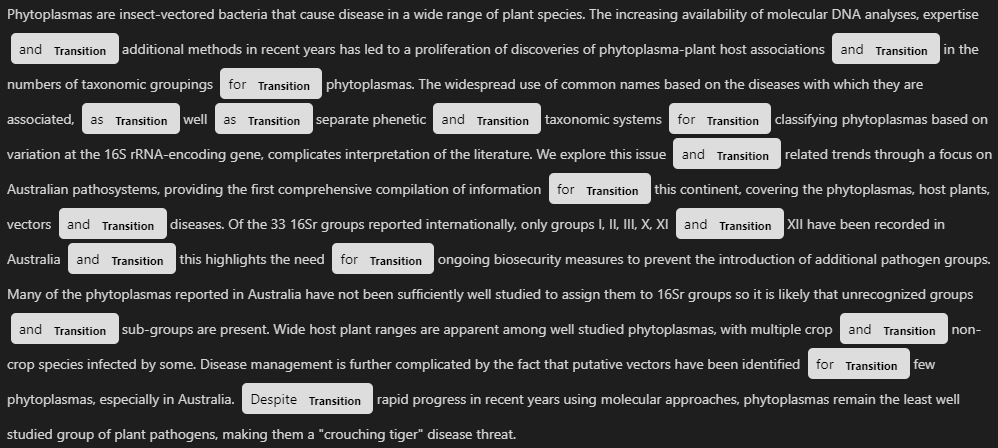
\includegraphics[width=0.45\textwidth,height=\textheight,keepaspectratio]{images/output.png}
\end{center}
\caption{Model output visualized via displacy}
\label{fig_output}
\end{figure}

\subsection{Assessing produced results and relevant metrics}
To gauge performance of our model versus pre-trained spaCy models, we would need to collect data and calculate certain metrics. This is done in three steps:

\begin{itemize}
    \item Run our new model alongside gold standard model on the same text
    \item Compare the results of these runs to generate confusion matrix
    \item Use confusion matrix to calculate metrics
\end{itemize}

\begin{figure}[htbp]
\begin{center}
    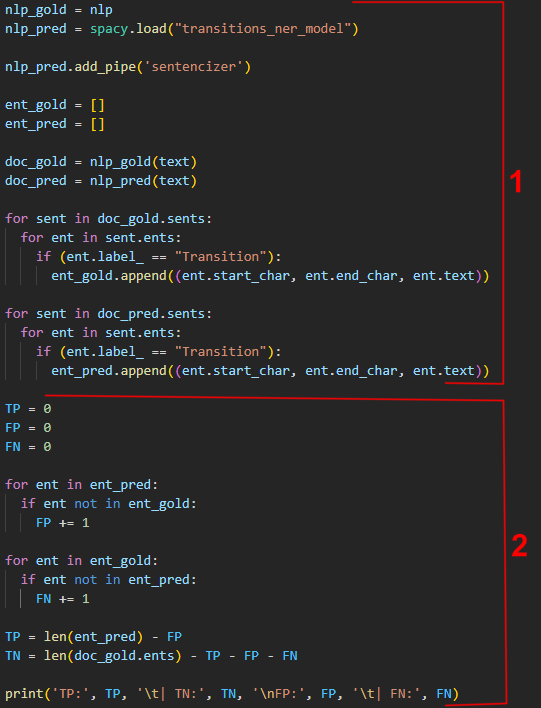
\includegraphics[width=0.45\textwidth,height=\textheight,keepaspectratio]{images/listing4.png}
\end{center}
\caption{Code for model assessment}
\label{fig_listing4}
\end{figure}

In the first step (block 1) we run both models on the text and collect all of the Transition entities that these models could find

In the second step we calculate values for the confusion matrix. They are as follows:

\begin{itemize}
    \item FP (false positive): number of non-Transition entities which the trained model classified as a Transition. To calculate this metric, we count entities which are found by our model but are not found by the gold standard model.
    \item FN (false negative): number of Transition entities which the trained model classified as a non-Transition or didn’t detect. To calculate this metric, we do the inverse - count entities detected by gold standard model, but not the trained model
    \item TP (true positive): number of Transition entities classified as Transition. To calculate this metric, we subtract FP from the total amount of positives (entities detected by trained model)
    \item TN (true negatives): number of non-Transition entities classified as non-Transition (or undetected). To calculate this, we subtract FP, FN and TP from the total amount of entities (number of entities detected by gold standard model)
\end{itemize}

\section{Evaluation and Discussion}

To evaluate our model, it's not enough to just use a confusion matrix. Instead we will accuracy, precision, recall and F1 metrics, which are accepted by scientific community and are commonly used to evaluate performance of various algorithms, such as NLP, machine learning and information retrieval. 

These metrics are computed as follows:

\begin{itemize}
    \item Accuracy: shows how accurate our model is in general (that is, how many entries did we correctly label out of all entries)
    \[
    Accuracy=\frac{TP+FN}{TP+TN+FP+FN}
    \]
    \item Precision: shows how likely it is for a positive predicted by our model to actually be a true positive (in other words, how many of entities labeled as transitions are actually transitions)
    \[
    Precision=\frac{TP}{TP+FP}
    \]
    \item Recall: shows how much out of all positives were detected by our model (that is, how much of true positives were labeled as such, as opposed to false negatives)
    \[
    Recall=\frac{TP}{TP+FN}
    \]
    \item F1: F1 is a harmonic mean between precision and recall. In application, it is similar to accuracy, but performs better in case of uneven class distribution (for example, large number of true negatives, which is true for this particular test) or uneven cost of false negatives versus false positives. Overall, it provides more balanced score of overall model performance.
    \[
    F1=2\times\frac{Precision \times Recall}{Precision+Recall}
    \]
\end{itemize}

For the final evaluation, values for confusion matrix are presented in the table \ref{tab:eval-1}. All the values were calculated based on a 500,000 character long data set created out of scientific paper abstracts.

\begin{table}[htbp]
\caption[Confusion matrix]{Confusion matrix} \label{tab:eval-1} 
\begin{center}
\begin{tabular}{|c|c|c|}
\hline
& Positive & Negative\\
\hline
\multicolumn{3}{@{}l}{} \\
\hline
True & 4388 & 3742\\
False & 283 & 953\\
\hline
\end{tabular}
\end{center}
\end{table}

Calculated metric values are provided in table \ref{tab:eval-2}.

\begin{table}[htbp]
\caption[Calculated metric values]{Calculated metric values} \label{tab:eval-2} 
\begin{center}
\begin{tabular}{|c|c|c|}
\hline
& Raw value & Approximated \% value\\
\hline
\multicolumn{3}{@{}l}{} \\
\hline
Accuracy & 0.8680333119795003 & 86.8\%\\
Precision & 0.9394134018411475 & 93.94\%\\
Recall & 0.8215689945703052 & 82.16\%\\
F1 & 0.8765481422293248 & 87.65\%\\
\hline
\end{tabular}
\end{center}
\end{table}

As we want to detect as much of transitions present in the text as possible, we want to minimize false negative metric. We can evaluated how well our model performed on that using recall metric. While the value of ~82\% is relatively high, based on this metric our model has room for improvement. 

This is also shown (though to a lesser degree) by our F1 metric. It is relatively high, and it's specifically applicable to our particular case: there are both uneven class distribution with large amount of true negatives and uneven weights of errors (as we would much rather see false positives, which might be transitions not considered while training initial model, than false negatives, which would mean that we missed a transition that our model should've known about and successfully detected).

Considering the relatively small size of the training data (comprised of approximately 11000 characters), we can conclude that overall the performance of the model was a success. With all of the metrics being greater than 80\%, the result is mostly agreed upon to signify a successful model performance (based on the papers reviewed in section "Literature Review").

However, there are still certain ways to improve model performance. For example, we can train it on a larger amount of data or increase initial transition word dataset. Methods to improve model's performance are discussed in detail in the following chapter.

\section{Conclusion}

A lot of current projects require processing raw text in some way. While previously main ways to do this were manual processing and text mining, with the recent rapid development of neural networks, NLP became another viable approach to such tasks. We confirmed that with an existing body of works which successfully implemented NLP for their needs, and developed our own solution to a problem that was not previously covered: detection of transition words in a text.

This model is usable in a variety of different applications:
\begin{enumerate}
    \item For educational purposes - it can be used as a tool that detects transitional words in a medium such as thesis papers or academic writing in general. As the model is trained on academic texts already, it can also provide a transitional word that will fit certain context both stylistically and contextually. This way, student can either get feedback on chosen transitional words or get a suggestion of one. In both cases, this would provide an opportunity to educate students on academic writing
    \item For proofreading assistance - if the user doesn't require suggestions for transitional words, this model can still be used for text analysis. It can provide useful data, such as usage by word (which can, in turn, be used to eliminate potential over-usage of certain words or repetitions)
    \item Data analysis - model can also be used to analyze texts for certain trends - for instance, it can be used to detect which transitional words are used more or less often, as well as new emerging transitional words (which can be useful for linguistic research purposes)
\end{enumerate}

Overall, this model successfully performed its function: it detected most of transition words and, even more importantly, successfully detected some tokens that exhibit properties of a transition word while not being in the initial set (one particularly notable example being the token "/" in constructions such as 'varied with mode/site of delivery'). However, as recall metric denotes that our model missed about 1 in 5 transition words, it would have to be improved in the future. There are several approaches, all of which will be taken in later development:

\begin{enumerate}
    \item Increase the transitional word data set: if we do that, we can reduce the number of false positive entries by including some of the transitional words that were detected, but weren't considered while creating initial data set.
    \item Increase the amount of training data: model was trained on a relatively small hand-crafted data set. In the final stages of model development, a bigger data set usable for training was found, but was only utilized in the evaluation of the model. Later on, the model can be trained on this data set as well.
    \item Employ customized modules: for instance, we can modify POS (part of speech) module and implement it to remove words which couldn't possibly be a transition word. For example, if we conclude that there are no adjectives in our transition words, we can exclude them as negatives later on, which would improve accuracy of our model.
    \item Implement feedback functionality: in certain cases, we can ask user to mark certain transitional words as correct or incorrect. This would be most fitting to use with a low-confidence results. Data collected that way could be used to improve the model as well as potentially creating individual user preferences.
\end{enumerate}

Additionally, following extensions and improvements to the existing program are considered for future development:

\begin{enumerate}
    \item Develop a GUI: currently, application only has a CLI. One of the first steps to improve its usability would be to introduce a GUI. This way, we can streamline part of the functionality (for example, providing text to analyze and exporting results) and enable future functionality (such as auto-correction, as described in the next point).
    \item Develop transition word proposal functionality: as we already have a model that can predict how fitting a word is to be a transition, we can later on extend the functionality to propose a transitional word based on a given position in sentence and the sentence itself. This, in turn, can be used in several different ways (i.e. automatic correction and word suggestion).
    \item Consider Information retrieval (IR) applications: IR could be employed by this algorithm in case of implementing additional functionality. In particular, we can use IR to compare multiple documents when we would offer the most fitting transitional word for a particular case. IR would help to compare submitted text to an existing text, which is either a text previously written by the same author (if our goal is to adhere to a particular author's style) or a document written with a specific style guidelines in mind (i.e. academic writing).
\end{enumerate}

\printbibliography[heading=bibintoc,title={Bibliography cited}]

\end{document}